\documentclass[aspectratio=169]{beamer}
\setbeamertemplate{footline}[frame number]
%\documentclass[aspectratio=169,notes=only]{beamer}
\usepackage{multicol}
\usepackage{wrapfig}
\usepackage{algorithmicx}
\usepackage{algpseudocode}
\usepackage{graphicx}
%\usepackage{subcaption} % cannot be used

\usepackage[english]{layout}
\usepackage[utf8]{inputenc}
\usepackage[english]{babel}
\usepackage[T1]{fontenc}
\usepackage{amsmath, soul, color, multicol, type1cm, verbatim, latexsym, dsfont, float, listings,alltt,tikz, lmodern, textcomp}
\usepackage[official]{eurosym}
\usepackage[export]{adjustbox}
\usepackage[caption = false]{subfig}
%\usepackage{beamerthemesplit}
%\usetheme{Frankfurt}
\usecolortheme{lily}
%\usefonttheme{structuresmallcapsserif}
\usefonttheme{professionalfonts}
\setbeamercovered{transparent}

\newcommand{\pluseq}{\mathrel{{+}{=}}}

%NeSI Colors <-------------------------------------------------------------------------------------
\usecolortheme{lily}
\usecolortheme[RGB={47, 68, 71}]{structure} 
\definecolor{nesidark}{HTML}{2F4447}
\definecolor{nesilight}{HTML}{CED9DF}
\definecolor{nesigrey}{gray}{0.7}
\definecolor{nesilightgrey}{gray}{0.98}
\definecolor{nesidarkgrey}{gray}{0.3}
\definecolor{nesiblue}{HTML}{2B9FC2}
\setbeamercolor{block title}{fg=black,bg=nesigrey}
\setbeamercolor{block body}{bg=nesilightgrey,fg=nesidarkgrey}
\setbeamercolor{block body alerted}{bg=white,fg=black}
\setbeamercolor{alerted text}{bg=white,fg=black}
\addtobeamertemplate{frametitle}{\vskip+1.2ex}{}
%NeSI Custom Code Hightlight <---------------------------------------------------------------------------------------
\lstdefinestyle{customcode}{
  belowcaptionskip=1\baselineskip,
  breaklines=true,
  xleftmargin=\parindent,
  showstringspaces=false,
  basicstyle=\ttfamily,
  keywordstyle=\bfseries\color{green!40!black},
  commentstyle=\itshape\color{purple!40!black},
  identifierstyle=\color{blue},
  stringstyle=\color{orange},
}
%NeSI Title <---------------------------------------------------------------------------------------
\setbeamerfont{title}{size=\huge}
\frenchspacing
\hyphenation{NeSI}
%NeSI Template parameters <-------------------------------------------------------------------------
\setbeamertemplate{blocks}[default]
\useinnertheme{circles}
\setbeamertemplate{title page}[default][center,rounded=false,shadow=false]
\newcommand\BackgroundPicture[1]{%
\setbeamertemplate{background}{%
\parbox[c][\paperheight]{\paperwidth}{%
\vfill \hfill \includegraphics[height=\paperheight]{#1}
\hfill \vfill
}}}

%\pagenumbering{arabic}

%Content Starts Here <-------------------------------------------------------------------------------
\title{\LARGE{Mimetic discretizations: new opportunities for pre- and post-processing}}
%\subtitle{Computational Science team}
\author{Alexander Pletzer (NeSI/NIWA), Wolfgang Hayek (NIWA/NeSI) and Jorge Bornemann (NIWA) \\
(alexander.pletzer@nesi.org.nz) \\
 Mathematical Sciences Institute \\
 Australian National University\\
 11 Dec 2017  }
\date{}

\begin{document}
\BackgroundPicture{NeSI/title.png}
\begin{frame}[plain]
  \vspace{+1.0cm}
  \titlepage
\end{frame}

% This will generate the outline. If you have several topics, uncomment the multicols 
\BackgroundPicture{NeSI/blank-01.png}

%%%%%%%%%%%%%%%%%%%%%%%%%%%%%%%%%%%%%%%%%%%%%%%%%%%%%%%%%%%%%%%%%%%%%%%%%%%%%%%%%%%%%%%%%%%%%%%
%%%%%%%%%%%%%%%%%%%%%%%%%%%%%%%%%%%%%%%% Some Examples %%%%%%%%%%%%%%%%%%%%%%%%%%%%%%%%%%%%%%%%
%%%%%%%%%%%%%%%%%%%%%%%%%%%%%%%%%%%%%%%%%%%%%%%%%%%%%%%%%%%%%%%%%%%%%%%%%%%%%%%%%%%%%%%%%%%%%%%
% List with bullets (itemize) <---
% The [<+-| alert@+>] will create a new slide for each element with highlighting 

\begin{frame}[t]
  \frametitle{National Institute for Water and Atmospheric Research Ltd (NIWA)}
  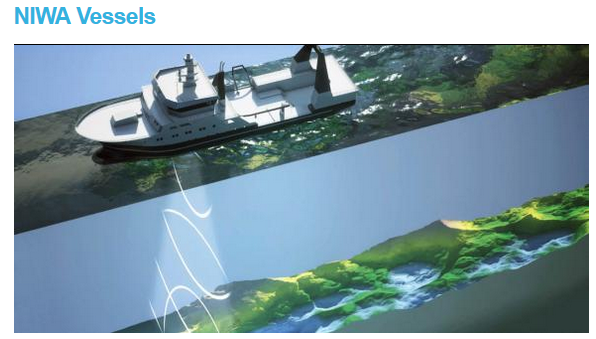
\includegraphics[width=0.8 \textwidth]{niwa2.png}
\end{frame}


\begin{frame}[t]
  \frametitle{Overview}
    \begin{block}{}
      \begin{itemize}%[<+-| alert@+>]
	  \item What are mimetic discretizations and why we care
      \item Why existing interpolation methods won't work
         \begin{itemize} \item Solution: make pre/post processing consistent with discretization \end{itemize}
      \item Addressing the problem using a differential form/exterior calculus approach
         \begin{itemize} \item 4 types of fields, 4 types of discretization and 4 types of interpolation 
                         \item the interpolation method is not a choice!
                         \end{itemize}
      \item Algorithms
         \begin{itemize} 
            \item Requires computing collision (intersection) of a grid with an object (point, line, area or volume)
         \end{itemize}
      \item Results
      \item Summary and further work
    \end{itemize}
  \end{block}
\end{frame}

\begin{frame}[t]
  \frametitle{What we mean by mimetic}
    \begin{block}{}
      \begin{itemize}%[<+-| alert@+>]
	  \item Discretization that preserves the mathematical properties of a field
            \begin{itemize}
            \item $\nabla \times \nabla = 0$ and $\nabla \cdot \nabla \times = 0$
            \item $\int \nabla \times E \cdot dS = \oint E \cdot d\ell$ and 
	  $\int \nabla \cdot D dV = \oint D \cdot dS$
            \end{itemize}
      \item Conserves quantities to near machine accuracy
           \begin{itemize}
              \item line integral 
              \item surface flux
              \item volume integral
           \end{itemize}
      \item Free of spurious modes and numerical pollution
            \begin{itemize}
              \item Mixed finite element methods based on H(curl) and H(div) elements
              \item Finite Difference Finite Time (FDFT) domain
              \item Discrete Exterior Calculus (DEC) methods
            \end{itemize}
      \item Bossavit (1989), Hiptmaier (1997), Hirani (2003), Arnold (2002), Gilette \& Bajaj (2010), Cotter \& Shipton (2014), Samtaney \& Mohamed (2015) 
    \end{itemize}
  \end{block}
\end{frame}

\BackgroundPicture{NeSI/divider-01.png}
\begin{frame}[fragile]{}
  \begin{center}
    \Huge{\textbf{Motivation}}
  \end{center}
\end{frame}
\BackgroundPicture{NeSI/blank-01.png}

\begin{frame}[t]
  \frametitle{Want answers to following questions}
    \begin{block}{How should we interpolate vector fields with staggered components?}
      \begin{itemize}%[<+-| alert@+>]
	  \item Arakawa C/D grids
      \item Components are on cell faces or edges
      \item Arises in computational fluid dynamics and electromagnetics
    \end{itemize}
  \end{block}
  \begin{tabular}{lr}
      % after \\: \hline or \cline{col1-col2} \cline{col3-col4} ...
      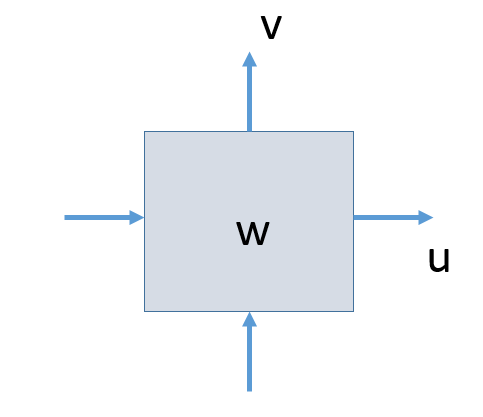
\includegraphics[width=30mm]{uvArakawaC.PNG} &               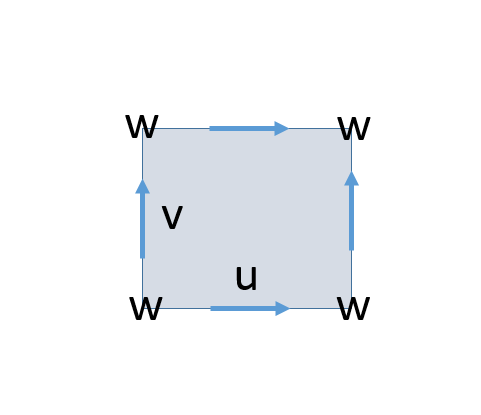
\includegraphics[width=30mm]{uvArakawaD.PNG} \\
      {Arakawa C-grid} & {Arakawa D-grid}  
\end{tabular}
\end{frame}

\begin{frame}[t]
  \frametitle{}
    \begin{block}{Can we unify existing interpolation methods?}
      \begin{itemize}%[<+-| alert@+>]
	  \item Linear, used since Babylonian times (2000-1700 BC)
      \item Conservative or area weighted, used in climate studies to enforce conservation
      \item In both cases the interpolation weights are ratios of areas (volumes)
      \item When is bilinear applicable and when should one use conservative? 
      \item Should vector fields with staggered components use bilinear or conservative? Or something else?
    \end{itemize}
  \end{block}
  \begin{tabular}{lr}
      % after \\: \hline or \cline{col1-col2} \cline{col3-col4} ...
      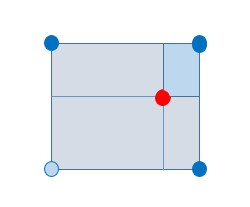
\includegraphics[width=30mm]{bilinear.png} &               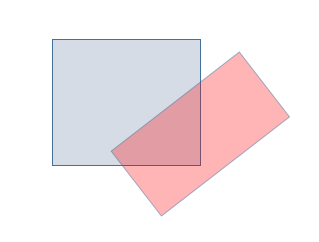
\includegraphics[width=30mm]{conservative.png} \\
      {Bilinear} & {Conservative}  
\end{tabular}
\end{frame}

\begin{frame}[t]
  \frametitle{}
  \begin{block}{How to handle curvilinear grids with non-orthogonal cells?}
  \end{block}
    Example: cubed-sphere grid
    \begin{itemize}
      \item Project grids on the surface of a cube onto a sphere
      \item Six logically rectangular grids (cannot be represented as a single structured grid)
      \item No pole-like singularity but some distortion where three tiles meet 
    \end{itemize}
  \begin{center}
    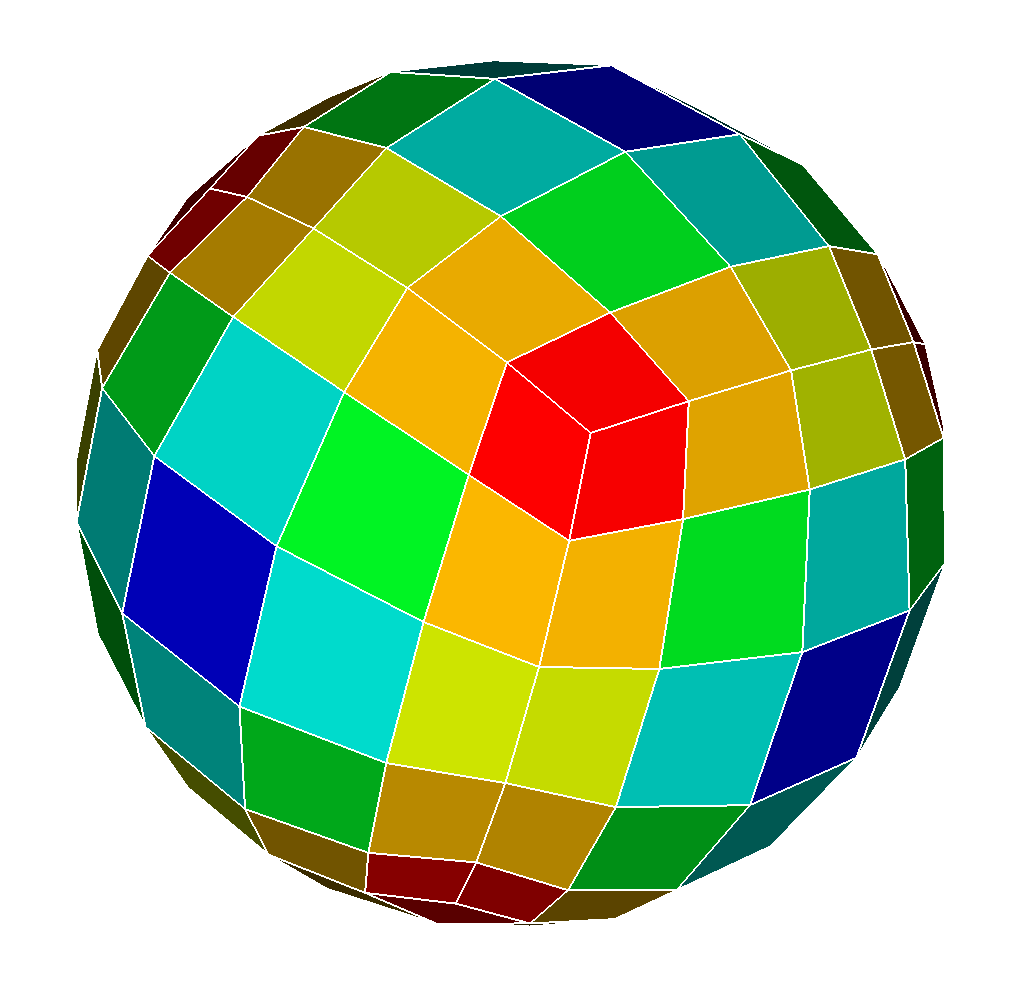
\includegraphics[width=0.35\textwidth]{cubedSphere.png}
  \end{center}
\end{frame}

\begin{frame}[t]
  \frametitle{}
  \begin{block}{How to compute surface fluxes?}
  \end{block}
  For example compute water fluxes across area
  \begin{center}
    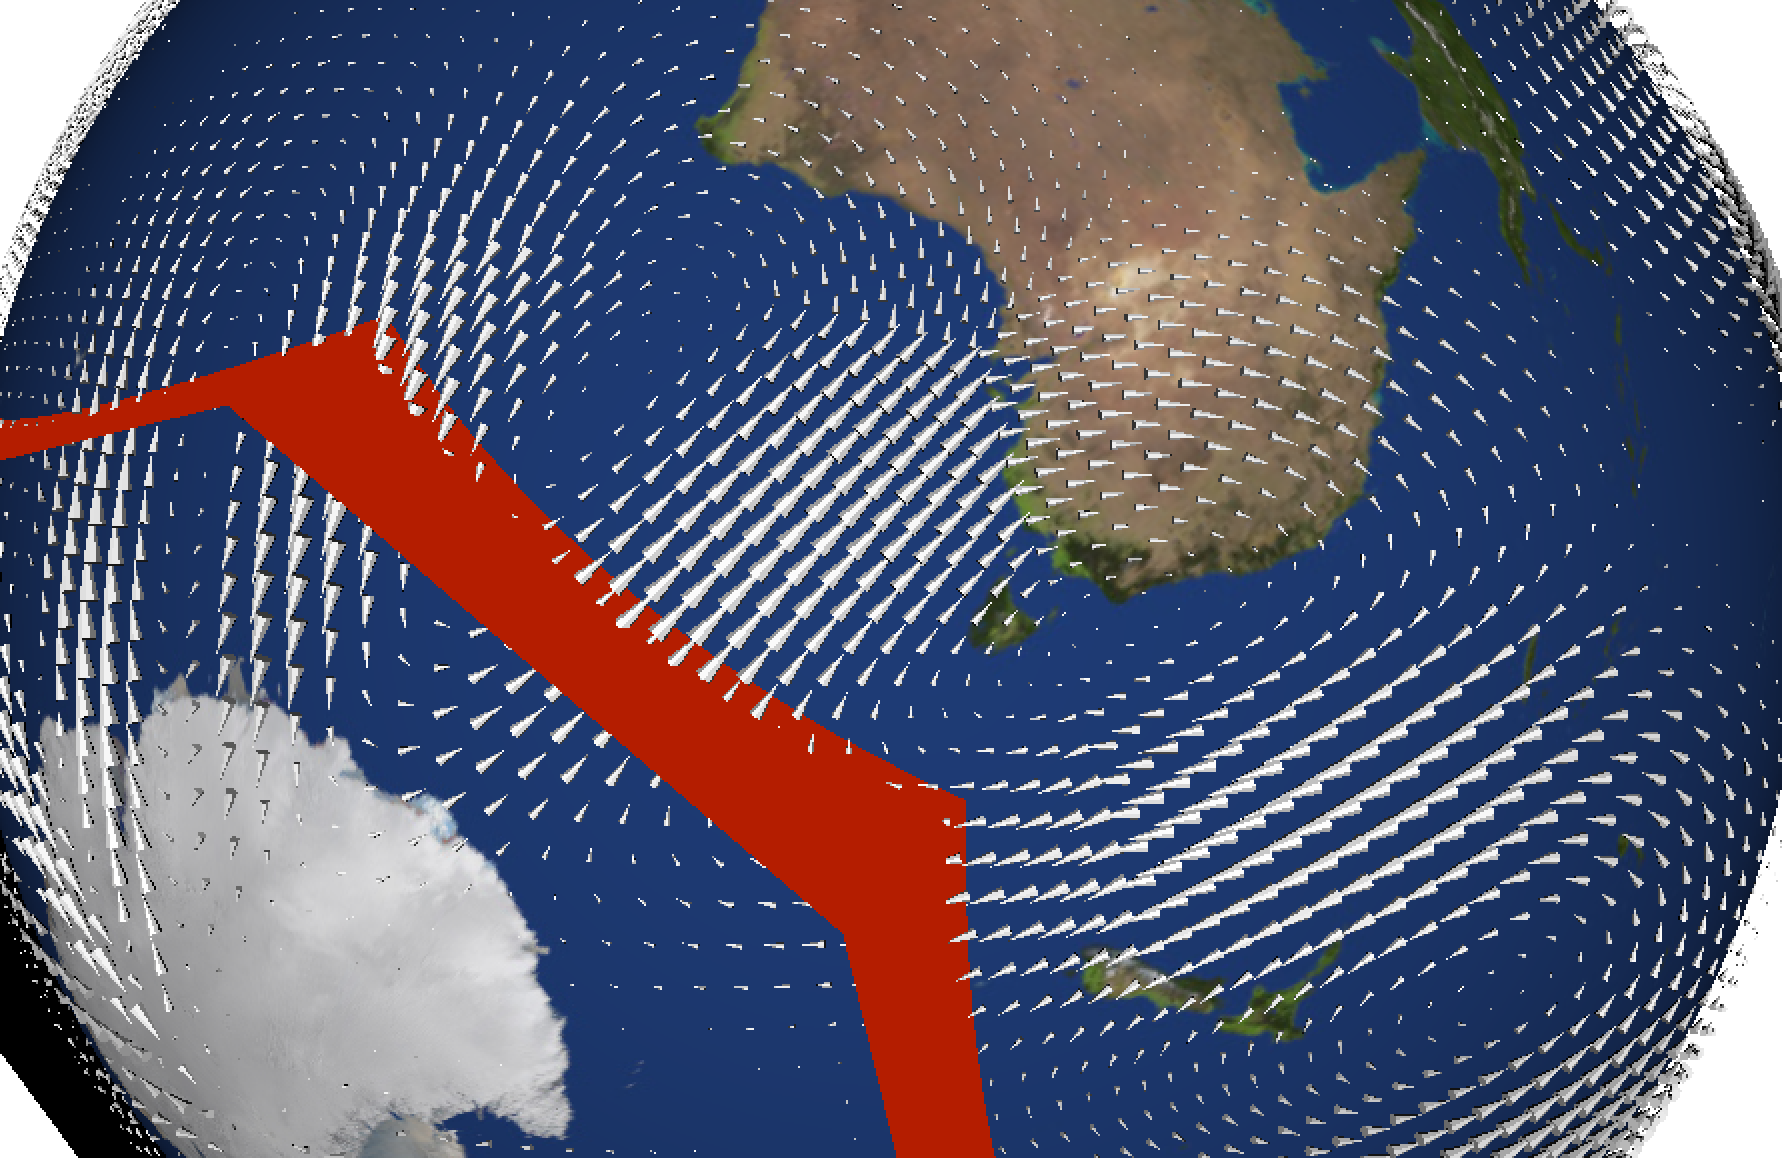
\includegraphics[width=0.6\textwidth]{fluxIntegral.png}
  \end{center}
  
\end{frame}

%\subsection{Divider examples}
\BackgroundPicture{NeSI/divider-02.png}
\begin{frame}[fragile]{}
  \begin{center}
    \Huge{\textbf{The type of field determines the discretization}}
  \end{center}
\end{frame}
\BackgroundPicture{NeSI/blank-01.png}

\begin{frame}[t]
  \frametitle{Some notation}
    \begin{block}{Coordinates}
      \begin{itemize}%[<+-| alert@+>]
      \item $\xi^i$ is curvilinear coordinate, $i = 1, 2, 3$
      \item $x$ is position (in physical space)
      \end{itemize}
    \end{block}
    \begin{block}{Wedge product}
       $\wedge$ (antisymmetric, like cross-product $\times$)
    \end{block}
    \begin{block}{Exterior derivative and contravariant bases}
      \begin{itemize}
        \item $d$ 
        \item similar to $\nabla$, $\nabla \times$, or $\nabla \cdot$
        \item $d \xi^i$ is basis function $\leftrightarrow \nabla \xi^i$
    \end{itemize}
  \end{block}
\end{frame}

\begin{frame}[t]
  \frametitle{Why four types of fields?}
    \begin{block}{One derivative - 4 fields }
      \begin{itemize}%[<+-| alert@+>]
	  \item 0-form: $\alpha(x)$ (just a function of space, one component)
        \begin{itemize}
          \item appropriate for scalar fields that don't change under coordinate transformations
          \item Example: temperature
        \end{itemize}
      \item 1-form: $\beta = \sum_i \beta_i d\xi^i$, basis is $d \xi^1$, 3 components
        \begin{itemize}
          \item appropriate for vector fields
          \item Examples: electric field $E$ and induction $H$
        \end{itemize}
      \item 2-form: $\gamma = \sum_{i < j} \gamma_{ij} d\xi^i \wedge d\xi^j$, basis is $d\xi^i \wedge d\xi^j$, 3 components
         \begin{itemize}
          \item appropriate for pseudo-vector fields, obtained by applying cross product of 1-forms
          \item Examples: magnetic field $B$ and displacement field $D$
        \end{itemize}
   \item 3-form: $\omega = \omega_{123} d\xi^1 \wedge d\xi^2 \wedge d\xi^3$, basis is $d\xi^1 \wedge d\xi^2 \wedge d\xi^3$, one component
         \begin{itemize}
          \item appropriate for pseudo-scalar, density-like fields 
        \end{itemize}
    \end{itemize}
  \end{block}
\end{frame}

\begin{frame}[t]
  \frametitle{Discretized versions of the fields}
    \begin{block}{Association of form with cell elements}
      \begin{itemize}%[<+-| alert@+>]
	  \item 0-form: {\color{red} on nodes}
        \begin{itemize}
          \item $\int \alpha = \alpha$ (integral is a no op)
        \end{itemize}
      \item 1-form: {\color{red} on edges}
        \begin{itemize}
          \item $\int \beta$ is a line integral
        \end{itemize}
      \item 2-form: {\color{red} on faces}
        \begin{itemize}
          \item $\int \gamma$ is a surface integral
        \end{itemize}
      \item 3-form: {\color{red} cell centred}
        \begin{itemize}
          \item $\int \omega$ is a volume integral
        \end{itemize}
    \end{itemize}
  \end{block}
  \begin{block}{Differential forms like to be integrated}
  \end{block}
\end{frame}

\begin{frame}[t]
  \frametitle{}
    \begin{block}{Ordering of vertices determines orientation of line, surface, volume}    
  \begin{center}
    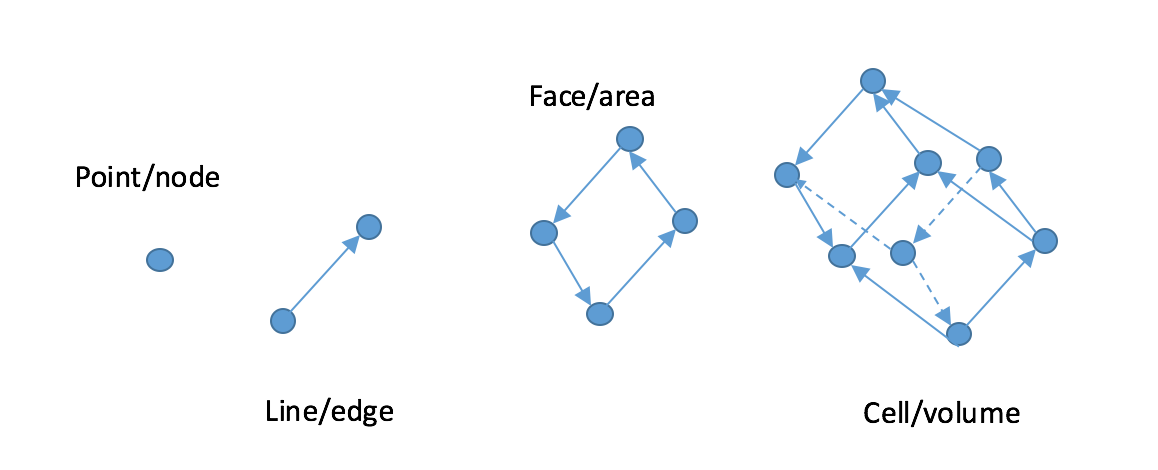
\includegraphics[width=0.8\textwidth]{orientedManifolds.png}
  \end{center}
  \end{block}
\end{frame}

\begin{frame}[t]
  \frametitle{One rule for $\nabla \times \nabla = 0$ and $\nabla \cdot \nabla \times = 0$}
  \begin{block}{What it means to be mimetic (1): $d^2 = 0$!}
    \begin{itemize}%[<+-| alert@+>]
    \item $d \alpha^0 \leftrightarrow \nabla \alpha$
    \item $d \beta^1 \leftrightarrow \nabla \times \beta$
    \item $d^2 \alpha^0 \leftrightarrow \nabla \times \nabla \alpha = 0$
    \item $d \gamma^2 \leftrightarrow \nabla \cdot \gamma$
    \item $d^2 \beta^1 \leftrightarrow \nabla \cdot \nabla \times \beta = 0$
    \end{itemize}
  \end{block}
  \begin{block}{What it means to be mimetic (2); divergence, Stokes' and gradient theorems}
   $\int_M d \alpha^k = \oint_{\partial M} \alpha^k$
  \end{block}
\end{frame}

\begin{frame}[t]
  \frametitle{It's easy to write integral of a differential form in any coordinate system}
  \begin{block}{Pullback of a differential form introduces Jacobian}
     \begin{itemize}
       \item $\int \beta(\xi) d\xi = \int \beta(t) \frac{d\xi}{dt} dt$ ($t$ is line parametrization)
       \item $\int \gamma(\xi) d\xi^1 \wedge d\xi^2 = \int \gamma(\eta) \det \left( \frac{\partial\xi}{\partial \eta} \right) d\eta^1 \wedge d\eta^2$ ($\eta^1$ and $\eta^2$ are surface parametrization)
       \item $\int \omega(\xi) d\xi^1 \wedge d\xi^2 \wedge d\xi^3 = \int \omega(\eta) \det \left( \frac{\partial\xi}{\partial \eta} \right) d\eta^1 \wedge d\eta^2 \wedge d\eta^3$
     \end{itemize}
  \end{block}
  \begin{block}{We will see in next section that the above are exactly what we need for interpolation.}
  \end{block}
\end{frame}

%\subsection{Divider examples}
\BackgroundPicture{NeSI/divider-04.png}
\begin{frame}[fragile]{}
  \begin{center}
    \Huge{\textbf{Interpolation}}
  \end{center}
\end{frame}
\BackgroundPicture{NeSI/blank-01.png}

\begin{frame}[fragile]{Generalizing ``interpolation''}
\begin{block}{Making interpolation work for nodal, edge, face and cell fields}
$\int f = \sum_i f_i \int_T \phi_i$
\begin{itemize}
\item $\phi_i$ is basis $k$-form, $k =$ 0, 1, 2 or 3
\item $T$ is target (point, line, area or volume)
\item $f_i$ is field integral over cell element $k$ (node, edge, face or cell)
\item $\int_T \phi_i$ is the interpolation weight
\item $i$ index runs over all the degrees of freedom (points, edges, faces etc., as appropriate)
\end{itemize}
\end{block}
\end{frame}

\begin{frame}[fragile]{Identifing cell elements for low order basis forms}

\begin{block}{$i = (i_1, i_2, i_3)$ with $i_j \in \{0, 1, \star\}$}
 \begin{itemize}
   \item 0 is low side
   \item 1 is the high side
   \item $\star$ element varies in this direction
   \item $(\star, \star, \star)$ is the cell
 \end{itemize}
 \begin{center}
   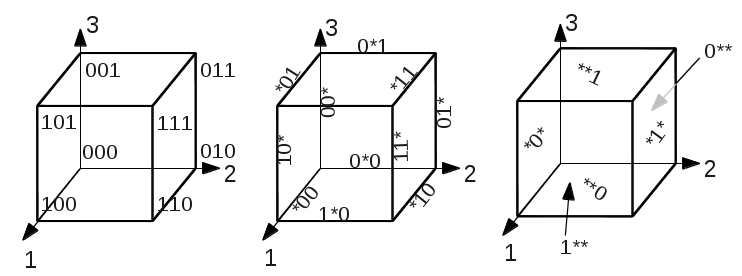
\includegraphics[width=0.7\textwidth] {gridElements.png}
 \end{center}
 \end{block}

\end{frame}

\begin{frame}[fragile]{Want the basis functions to satisfy orthogonality condition}

\begin{block}{$\int_i \phi_j = \delta_{ij}$}
 \begin{itemize}
   \item $i$ is cell element (node, edge, face, cell)
   \item $j$ is basis function index
   \item nodal bases are zero on all nodes expect one where it is one
   \item edge bases have zero integral on all edges except itself where it is one
   \item face bases have zero integral on all faces except itself where it is one
 \end{itemize}
 \end{block}

\end{frame}

\begin{frame}[fragile]{The $k = 0$ bases are the usual tent functions}

\begin{block}{}
\begin{itemize}
\item $\phi_{000} = (1-\xi^1)(1-\xi^2)(1-\xi^3)$
\item $\phi_{001} = (1-\xi^1)(1-\xi^2)\xi^3$
\item $\phi_{010} = (1-\xi^1)\xi^2(1-\xi^3)$
\item $\phi_{011} = (1-\xi^1)\xi^2 \xi^3$
\item $\cdots$
\item $\phi_{111} = \xi^1 \xi^2 \xi^3$
\end{itemize}
 \end{block}

\end{frame}

\begin{frame}[fragile]{The $k = 1, 2, 3$ bases basis forms}

\begin{block}{$k = 1$ bases are $H(curl)$ finite elements}
\begin{itemize}
\item $\phi_{00\star} = (1-\xi^1)(1-\xi^2) d\xi^3$
\item $\phi_{01\star} = (1-\xi^1) \xi^2 d\xi^3$
%\item $\phi_{10\star} = \xi^1 (1-\xi^2) d\xi^3$
%\item $\phi_{11\star} = \xi^1 \xi^2 d\xi^3$
\item $\cdots$
\item $\phi_{\star11} = \xi^2 \xi^3 d\xi^1$
\end{itemize} 
%\centering
%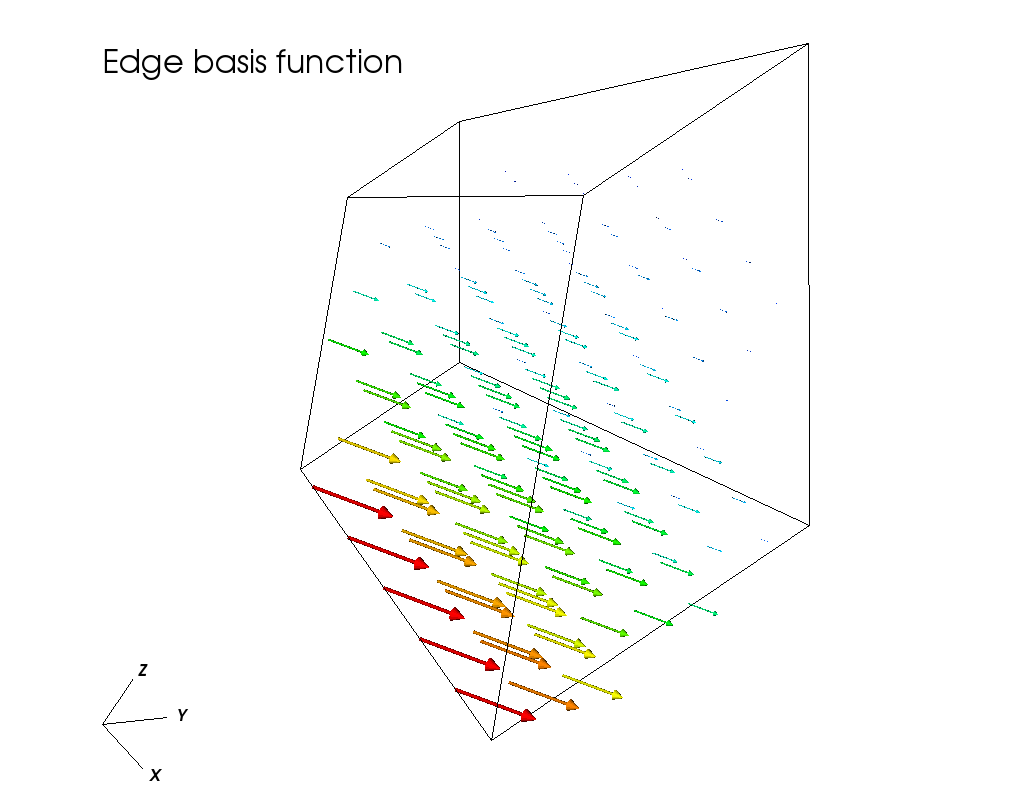
\includegraphics[width=0.3\textwidth]{hexEdge.png}
%1-form basis vanishes on opposite edge and is perpendicular to incident edges
 \end{block}
\begin{block}{$k = 2$ bases are $H(div)$ finite elements}
\begin{itemize}
\item $\phi_{0\star\star} = (1-\xi^1) d\xi^2 \wedge d\xi^3$
\item $\phi_{1\star\star} = \xi^1 d\xi^2 \wedge d\xi^3$
\item $\cdots$
\item $\phi_{\star\star1} = \xi^3 d\xi^1 \wedge d \xi^2 $
\end{itemize}
\end{block}
\end{frame}

\begin{frame}[fragile]{Observe how the $k = 1, 2$ bases satisfy the orthogonality condition}

  \begin{tabular}{lr}
      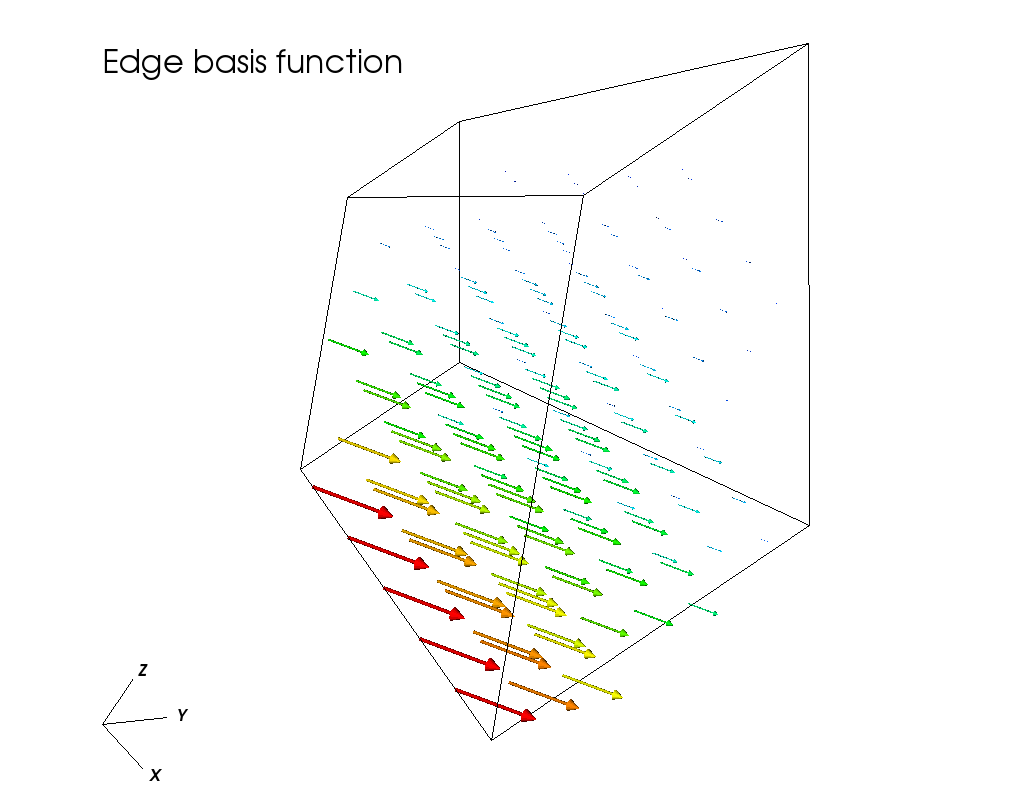
\includegraphics[width=50mm]{hexEdge.png} &                        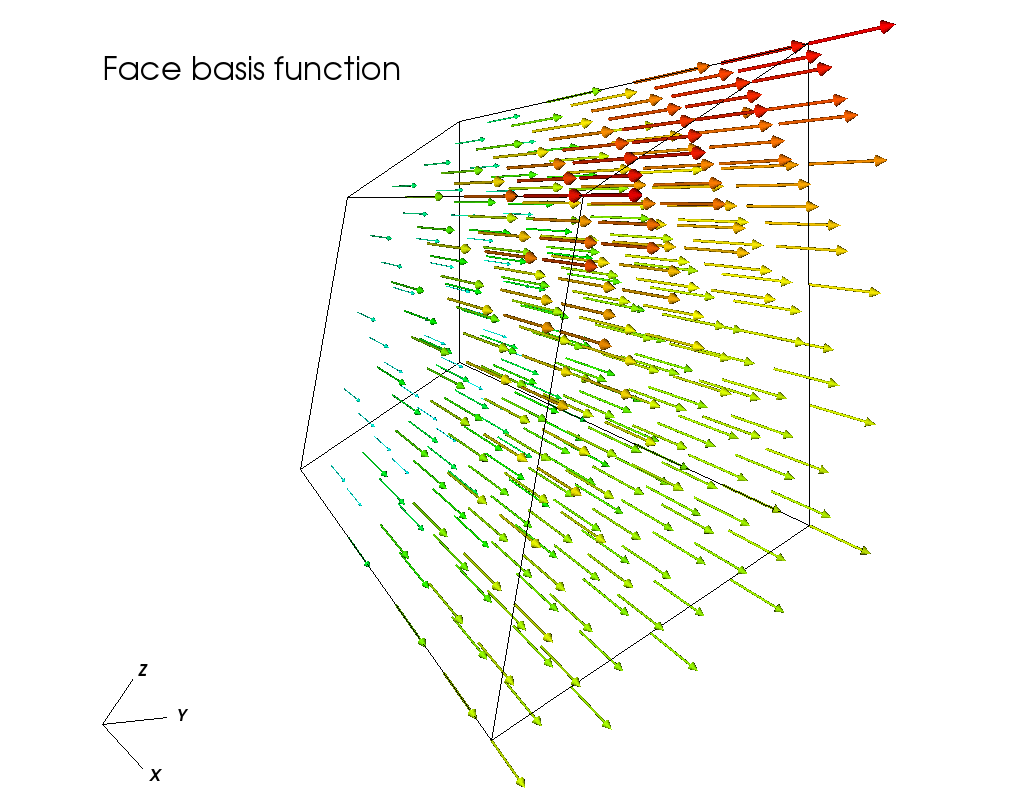
\includegraphics[width=50mm]{hexFace.png} \\
      {Edge basis is perpendicular } & {Face basis is tangent }  \\
      {to neighbouring edges} & {to neighbouring faces}
\end{tabular}


%\centering
%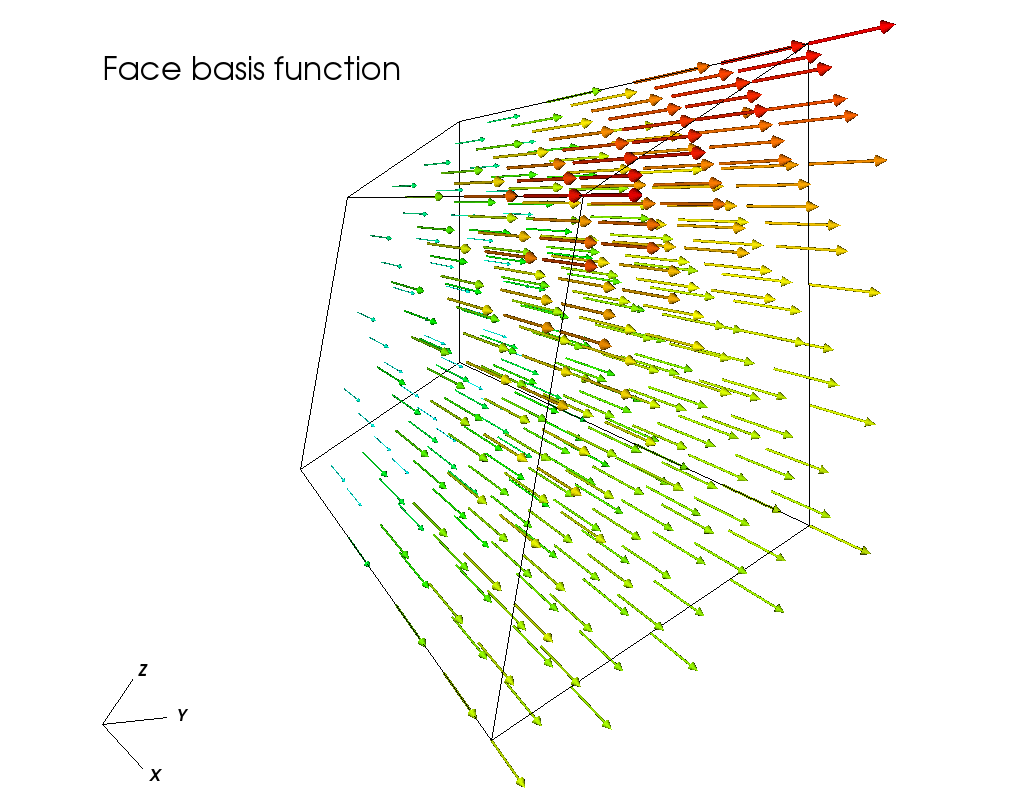
\includegraphics[width=0.3\textwidth]{hexFace.png}
% 2-form basis vanishes on opposite face and is tangent to incident faces
% \end{block}
\end{frame}

\begin{frame}[fragile]{Computing the interpolation weights}

\begin{block}{Assume target is a simplex}
$T:\lambda \rightarrow \xi = \xi_0 + \sum_{i=1}^k \lambda_i(\xi_i - \xi_0)$
 \end{block}
\begin{block}{Interpolation weight is the pullback, $\det(\partial \xi/\partial \lambda)$ is size of simplex in $\xi$ space}
$\int_T \phi = \int T^* \phi(\xi) = \int \phi(\lambda) \det(\partial \xi/\partial \lambda)$ independent of $\xi$ coordinate system!
 \end{block}
\begin{block}{For 1-form $(1 - \xi^1)\xi^2d\xi^3$ and $\xi = \xi_0 + \lambda (\xi_1 - \xi_0)$:}
$\int_T \phi = (x_1 - x_0) \int_0^1 d\lambda \phi(\xi_0 + \lambda(\xi_1 - \xi_0))$
 \end{block}
 \begin{block}{Integrals can be computed analytically for polynomial bases and target simplices}
 \end{block}
\end{frame}

\begin{frame}[fragile]{Computing intersection of grid with target}
\begin{block}{grid cells with target points, grid faces with target edges, grid edge with target faces, etc}
\centering
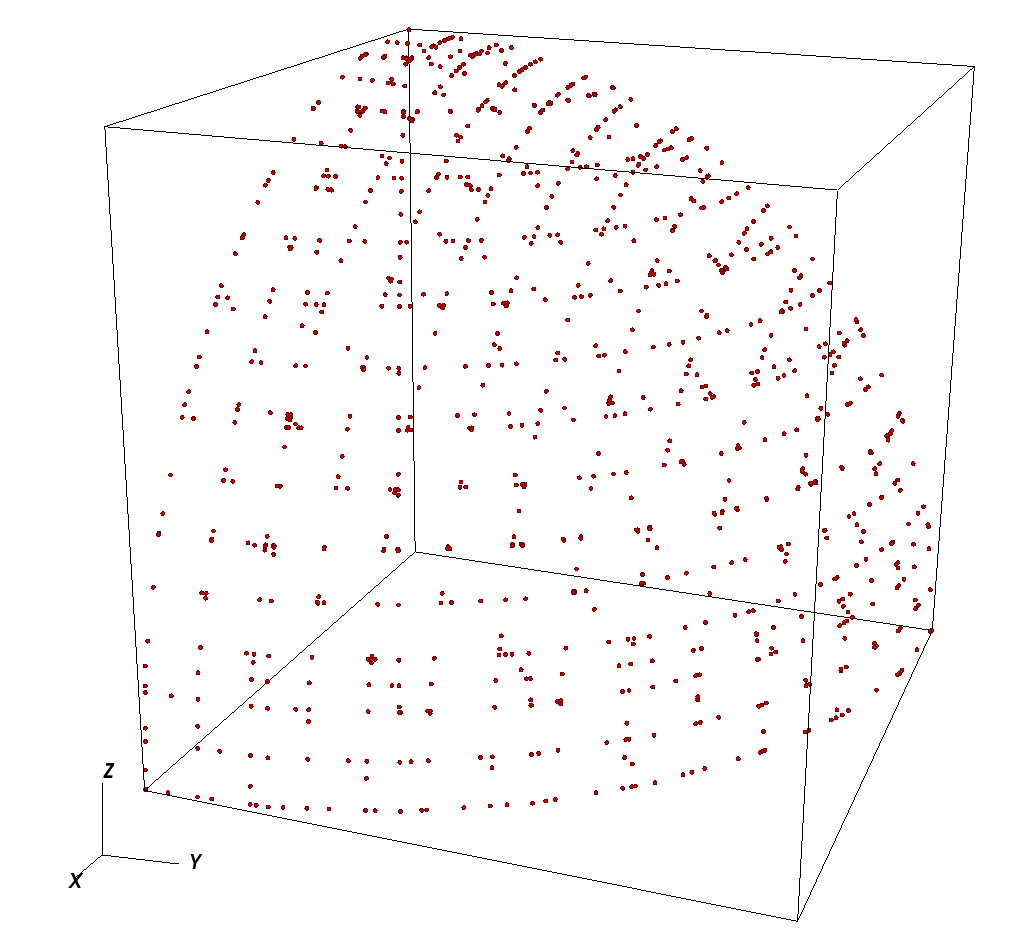
\includegraphics[width=0.6\textwidth]{pointIntersect.png}
\end{block}
\end{frame}

%\subsection{Divider examples}
\BackgroundPicture{NeSI/divider-04.png}
\begin{frame}[fragile]{}
  \begin{center}
    \Huge{\textbf{Results}}
  \end{center}
\end{frame}
\BackgroundPicture{NeSI/blank-01.png}

\begin{frame}[t]
  \frametitle{Divergence-free field in Cartesian coordinates}
  \begin{block}{Stream function}
  \begin{itemize}
  \item $v = dz \wedge d\psi$
  with stream function $\psi = \frac{\cos 2 \pi x}{4 \pi} + y^2$
  \item Closed surface fluxes $B$ and $C$ are exact 
  \item Flux on $A$ is exact because start/end points are nodes 
  \end{itemize}
\centering
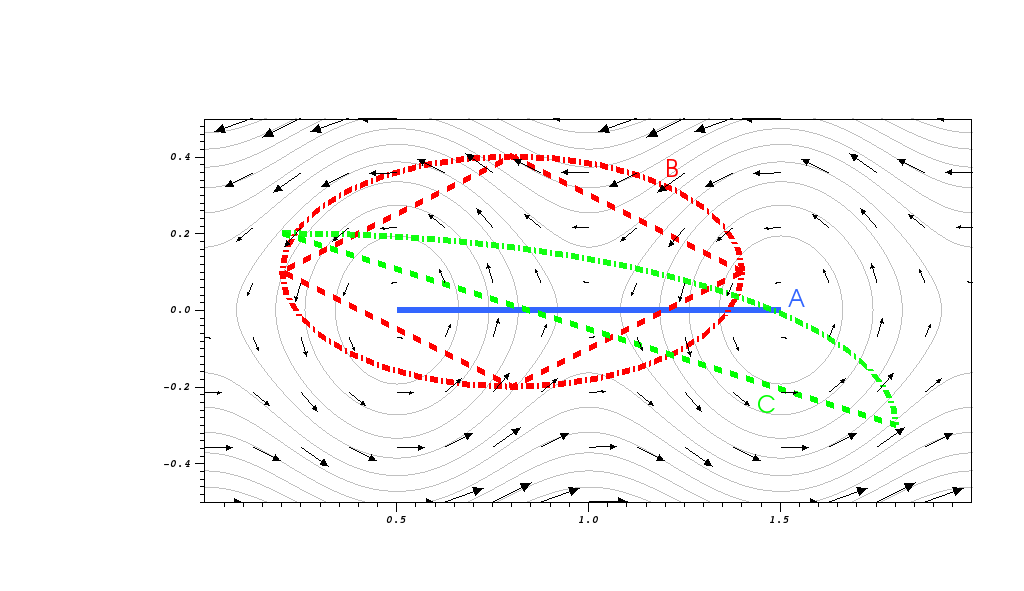
\includegraphics[width=0.6\textwidth]{flow.png}
\end{block}
\end{frame}

\begin{frame}[t]
  \frametitle{Vector field with singularity}
  \begin{block}{}
   $v = \frac{x dx + y dy}{2 \pi (x^2 + y^2)}$ chosen such that 
  $\oint v$ is 1 if contour contains singularity, 0 otherwise
  \end{block}
  
\begin{figure}[!htb]
\centering
\begin{minipage}{.49\textwidth}
  \centering
  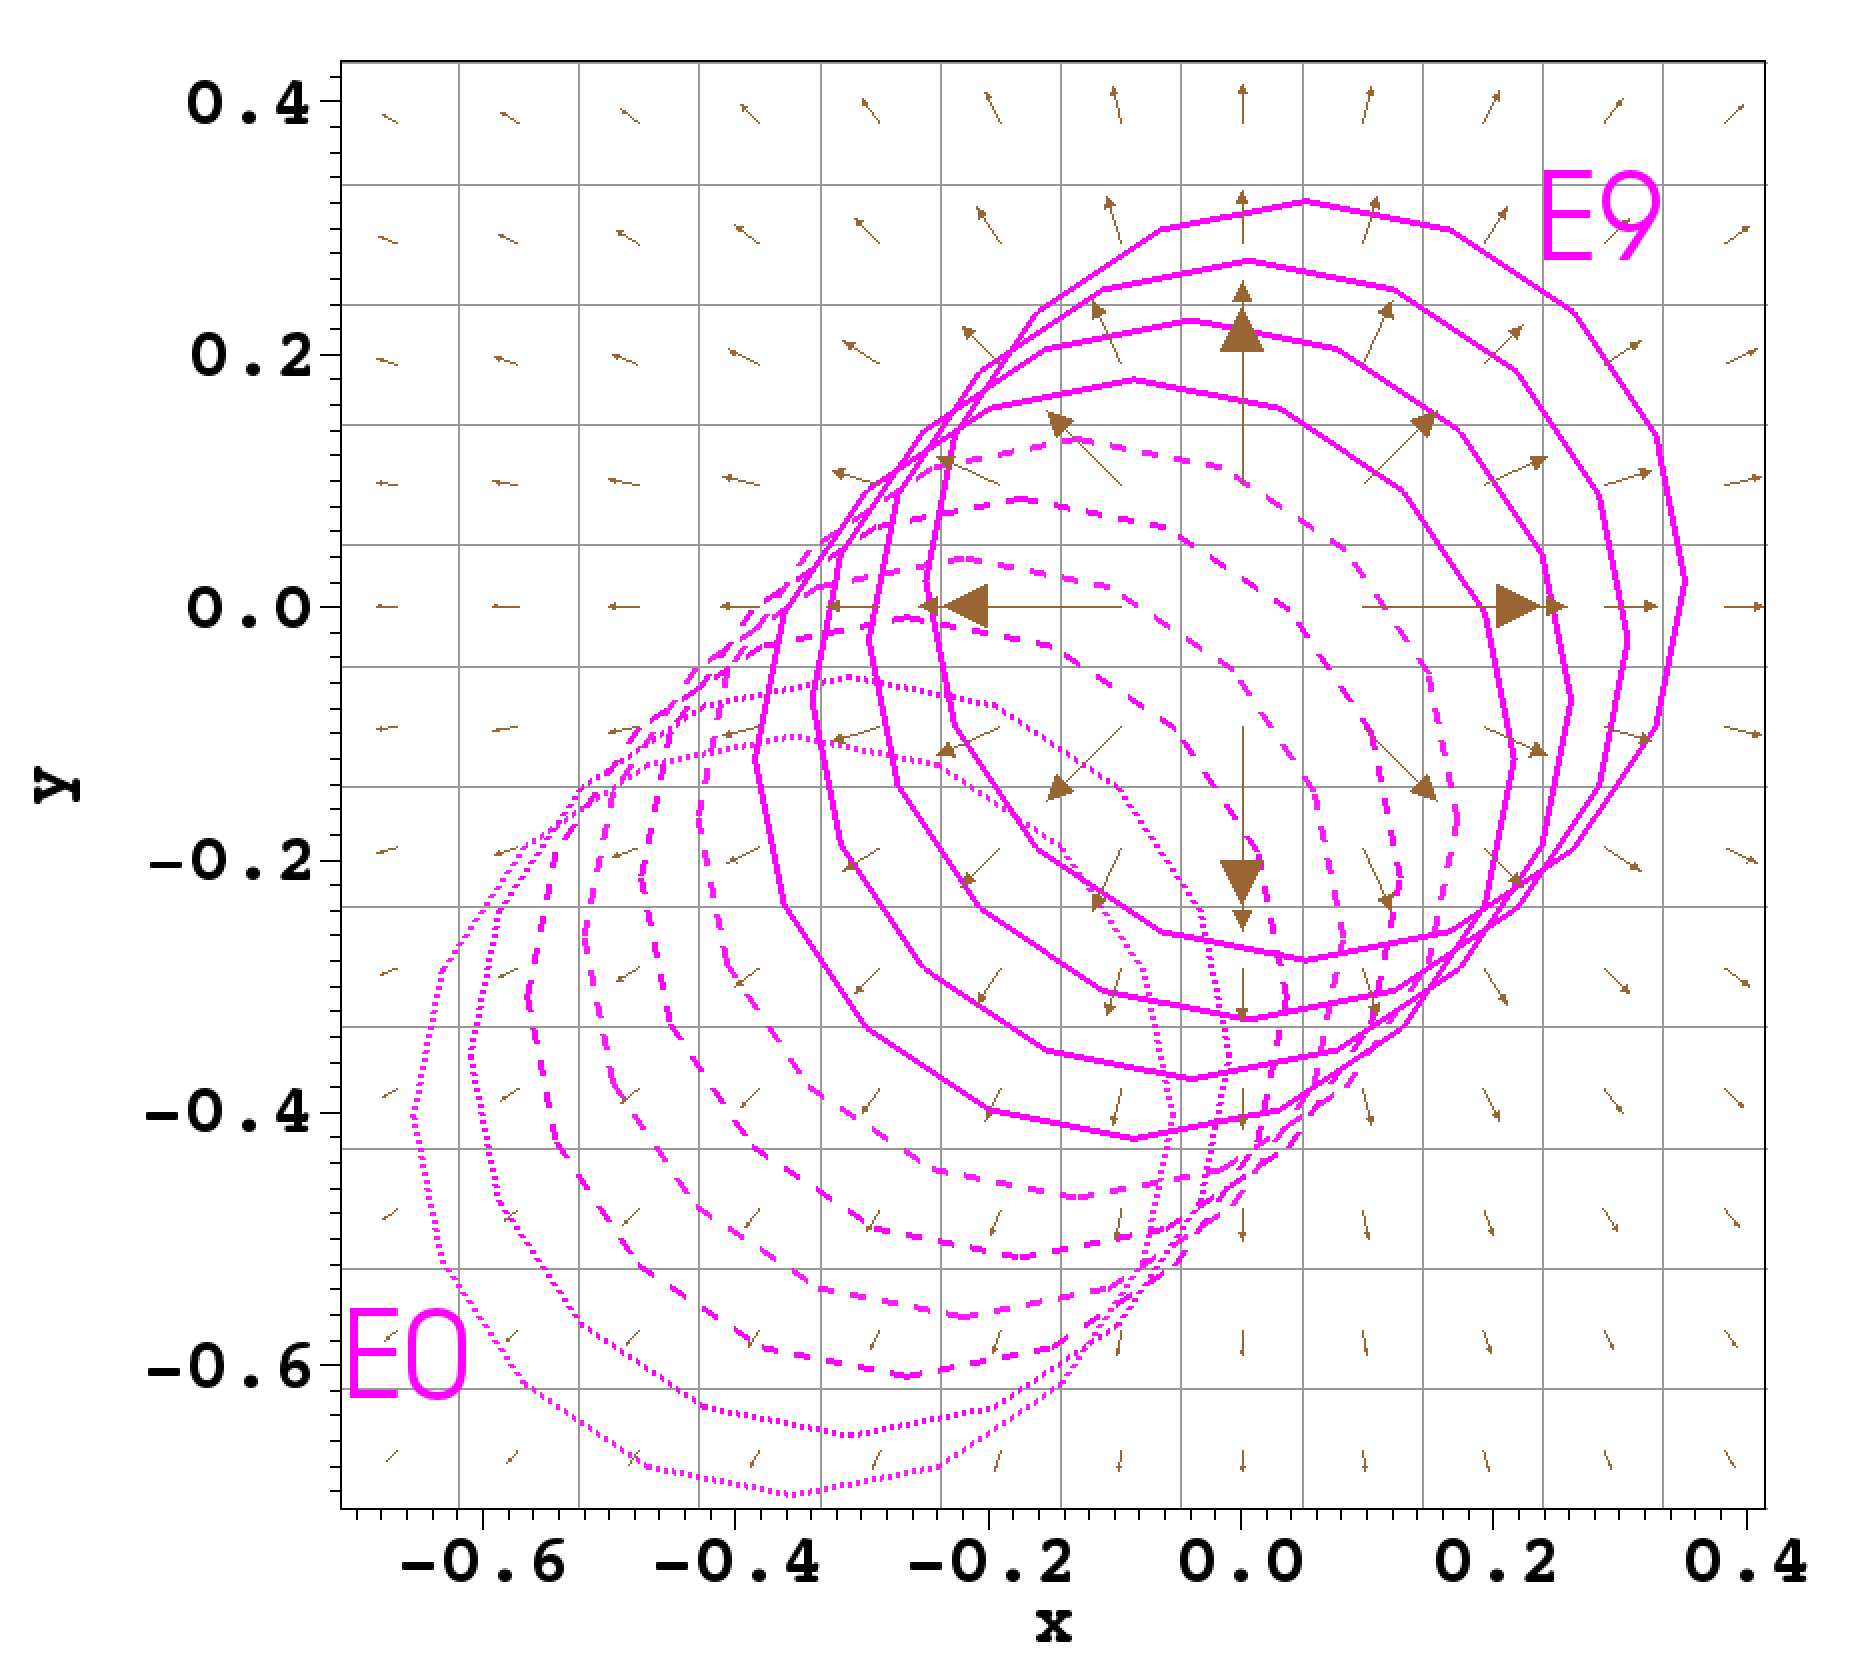
\includegraphics[width=.8\linewidth]{polar.png}
  \caption{Radial field}
\end{minipage}%
\begin{minipage}{.49\textwidth}
  \centering
  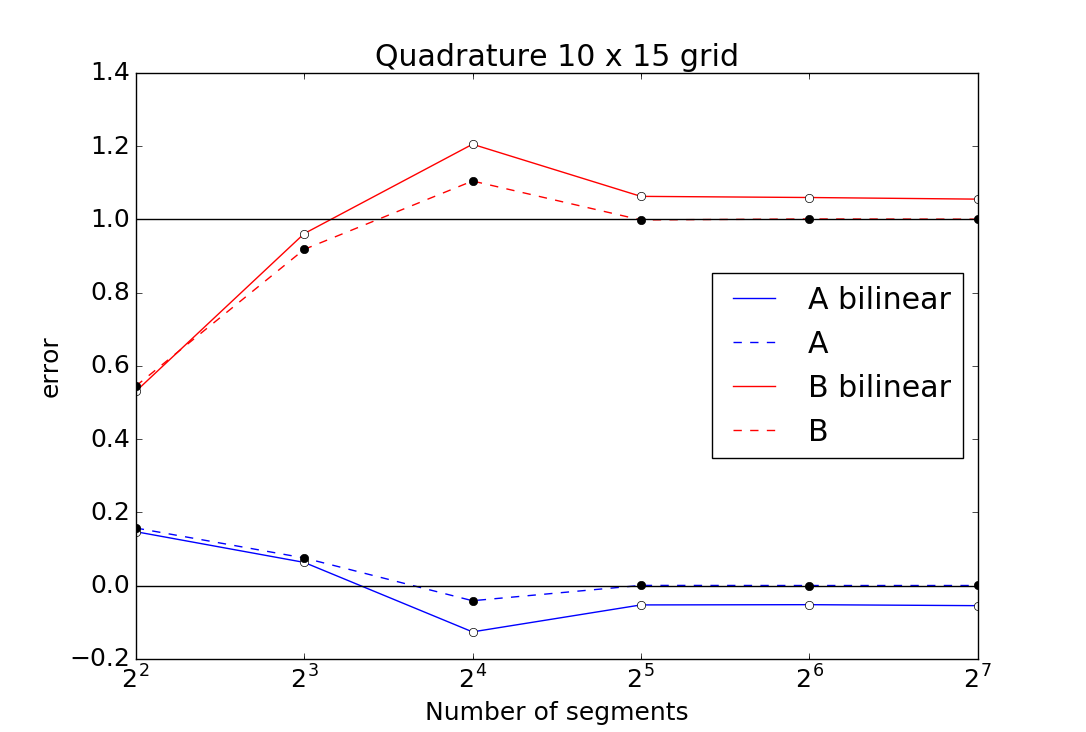
\includegraphics[width=.98\linewidth]{case2ErrorPlotAB.png}
  \caption{Numerical error}
\end{minipage}
\end{figure}
\end{frame}

\begin{frame}[t]
  \frametitle{Flux computation on the cubed sphere $v = d\psi \wedge dr$}
  \begin{block}{Error depends distance of start/end point from edge/face}
   \begin{itemize}
   \item $\psi$ is a function of longitude and latitude
   \item Some cells have 120 deg angle between edges
   \end{itemize}
  \end{block}
  
  \begin{tabular}{lr}
  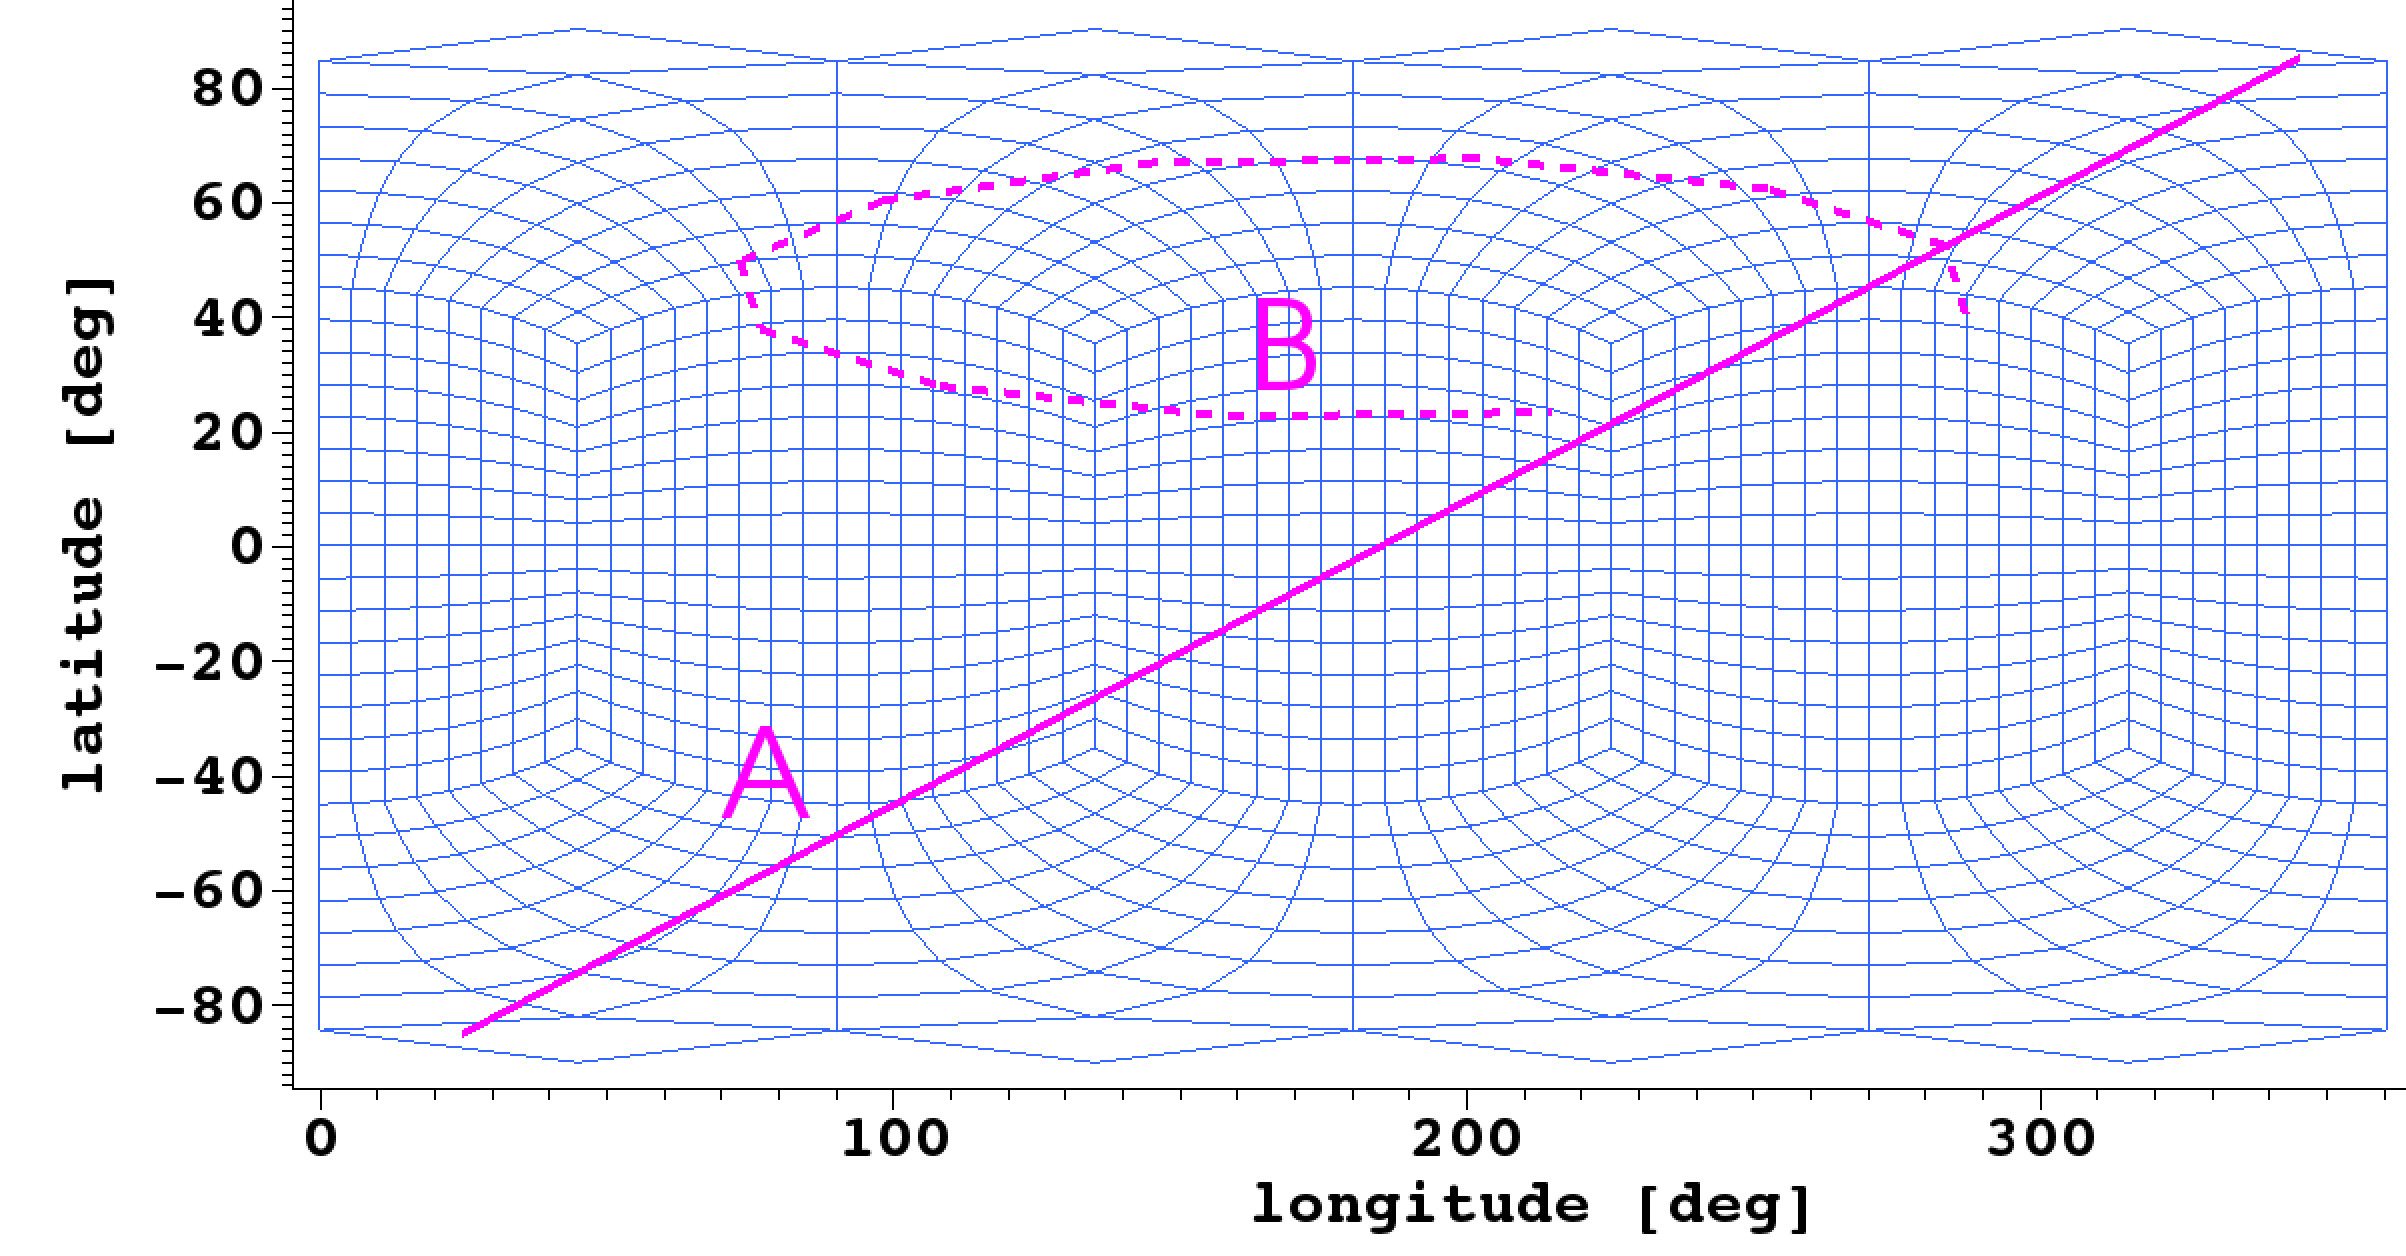
\includegraphics[width=30mm]{fluxOnCubedSphere.png} & 
  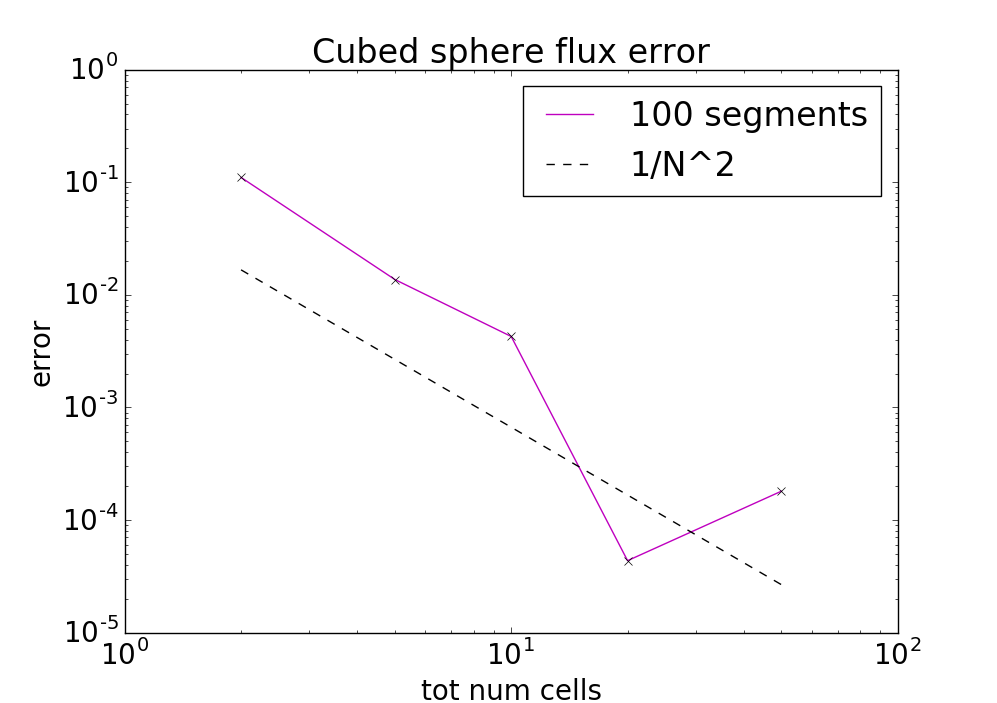
\includegraphics[width=50mm]{cubedSphereFluxError.png} \\
  {Integration path/surface} & {Error is $\sim 1/N^2$} 
  \end{tabular}
\end{frame}

\begin{frame}[t]
  \frametitle{Checking Maxwell's equations}
  \begin{block}{$F = E\wedge dt + B$. Faraday's law is $d F = 0$ (no charge). Plane wave.}
  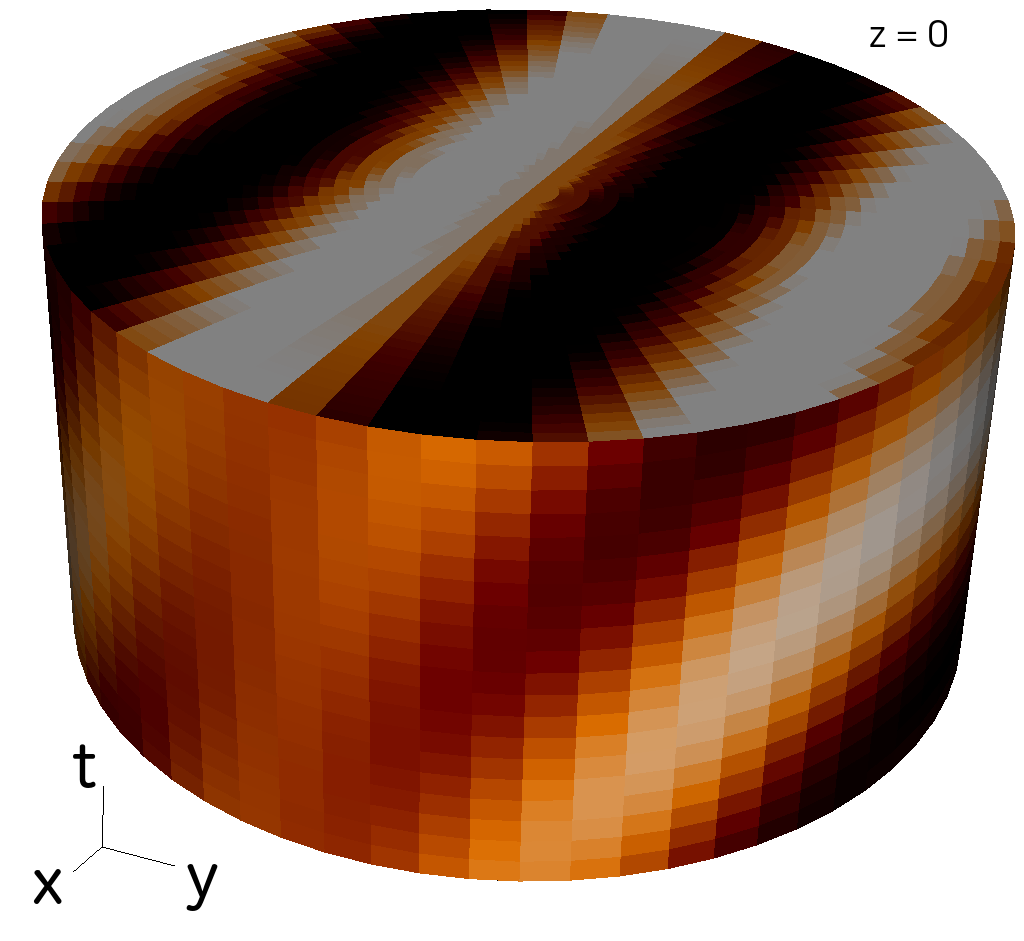
\includegraphics[width=70mm]{z0_0.png}
  \end{block}
\end{frame}

\BackgroundPicture{NeSI/divider-02.png}
\begin{frame}[fragile]{}
  \begin{center}
    \Huge{\textbf{Summary}}
  \end{center}
\end{frame}
\BackgroundPicture{NeSI/blank-01.png}

\begin{frame}[t]
  \frametitle{}
    \begin{block}{Different types of field $\leftrightarrow$ different staggerings}
      \begin{itemize}%[<+-| alert@+>]
	  \item nodal for scalar fields (e.g. temperature)
	  \item edge for vector fields (e.g. electric field)
	  \item face for pseudo-vector fields (e.g velocity)
	  \item cell for pseudo-scalar fields (e.g. density)
	  \item type of field $\rightarrow$ interpolation method
      \item field values set via cell, face and edge integrals (instead of vector field components)
	  \item who needs vector fields?
    \end{itemize}
    \end{block}
    \begin{block}{Masking and partially valid cells?}
	 Ok if taking account of partial cell, faces, edges when setting cell, face and edge integrals. Done!
  \end{block}
\end{frame}

\begin{frame}[t]
  \frametitle{Basis function extensions}
    \begin{block}{What about tetrahedra?}
      Similar approach except that the basis functions are Whitney's
    \end{block}
    \begin{block}{Higher order basis functions?}
    Initial work indicates that higher order basis functions can be used. These also satisfy the orthogonality condition $\int_i \phi_j = \delta_{ij}$
    on sub-cell edges, faces and cells. Quadratic elements effectively 
     split each cell into 8 sub-cells, each face into 4 sub-faces and each edge into 2 sub-edges. 
  \end{block}
\end{frame}

% End <-----------------------------------------------------------------------------------------
\BackgroundPicture{NeSI/blank-02.png}
\begin{frame}[plain]
  \begin{center}
  Goal is to apply the rigour of dynamical cores to pre- and post-processing tools. Overtime we expect the distinction between dynamical core
  and pre-/post-processing to diminish.
  \\
  
    \vspace*{+2cm}
    {\Huge Thank You}\\
    \vspace*{+1cm}
    
\includegraphics[width=100pt]{NeSI/nesi_logo.png}
  \end{center}
\end{frame}

\end{document} 